\section[Venue applications and scale]{Apply the Model: From a Ticket Queue to Fremont Street}
\label{sec:applications}
% Generated from venue_model/results.json; do not hand-edit.
\newcommand{\FMaxEta}{16.54}
\newcommand{\HMaxEta}{47.71}
\newcommand{\FTwb}{20.77}
\newcommand{\HTwb}{25.56}
\newcommand{\FCDrop}{8.00}
\newcommand{\HCDrop}{3.81}
\newcommand{\HWithFEta}{49.63}


Figure~\ref{fig:us-climate} places the sites in a national climate context. NASA POWER provides 77 geographic samples of July mean $T_a$, RH and pressure for 2001--2025 \cite{nasa-power}. We evaluate wet bulb at each paired mean state and interpolate the resulting depression over the contiguous states and Hawaii \cite{us-boundaries}. This is a climatological-state diagnostic, not an average of hourly cooling potential; the original design scenarios remain separate.

\begin{figure}[!ht]
\centering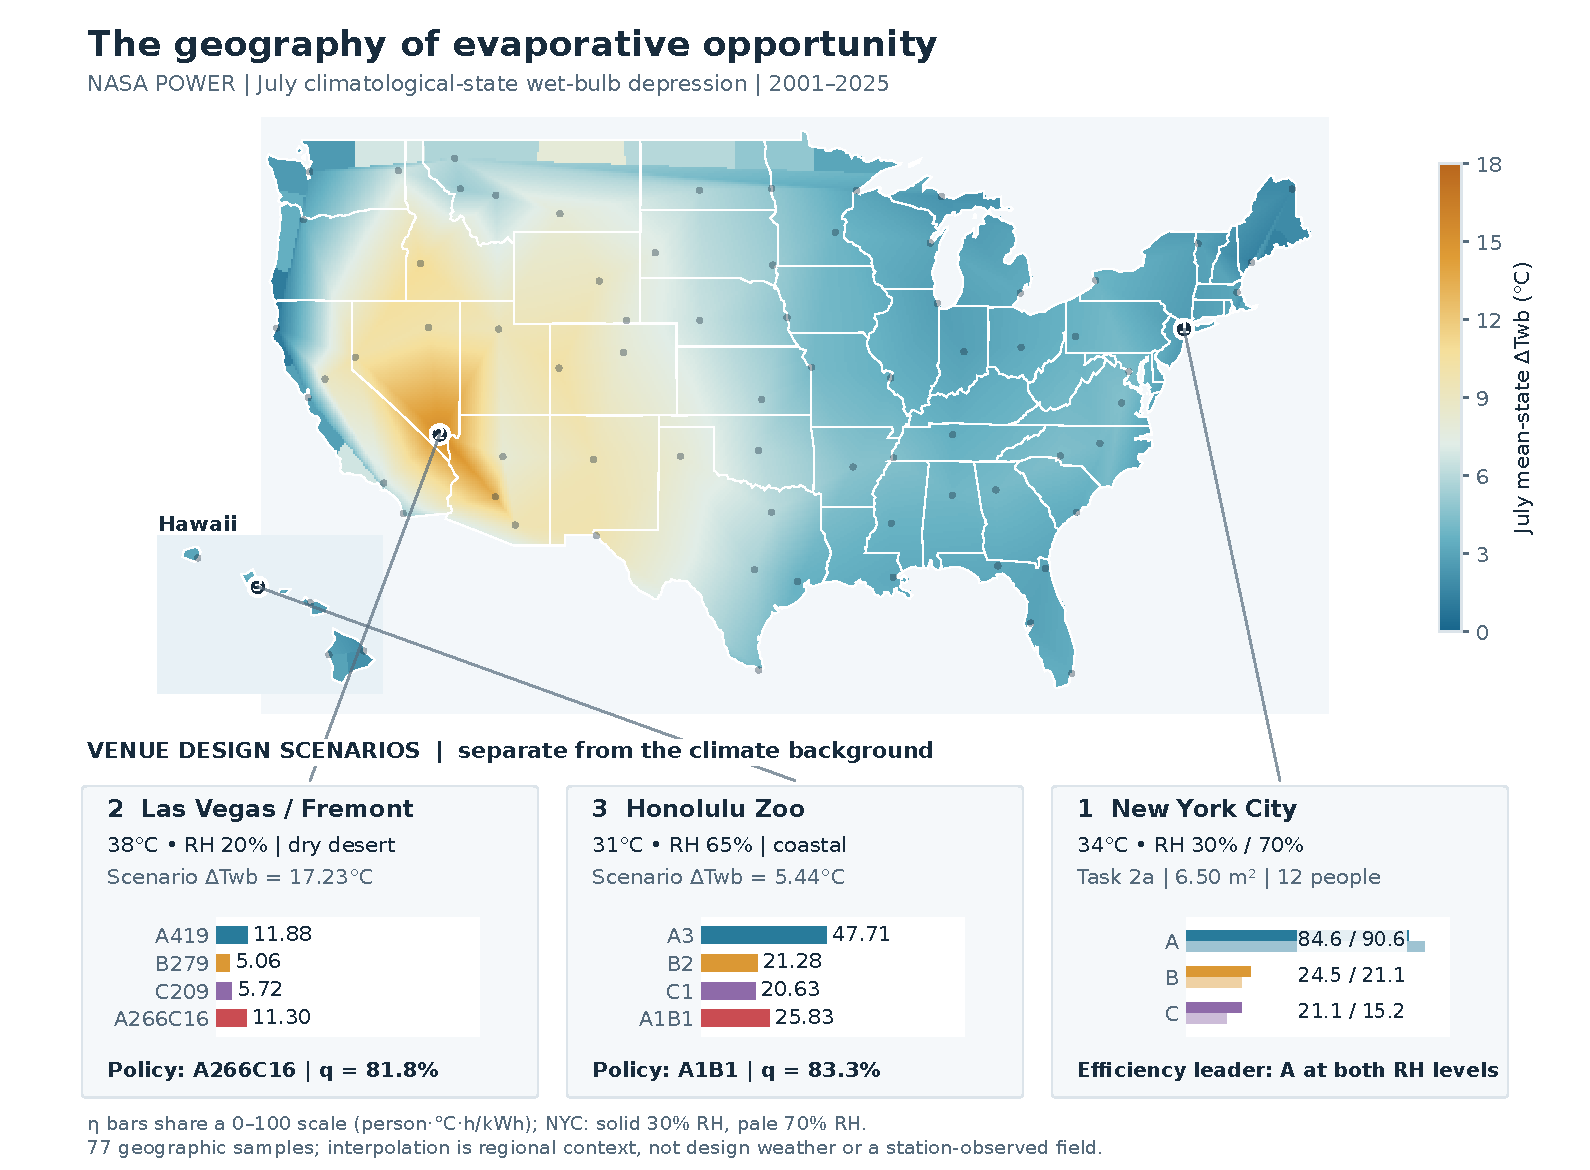
\includegraphics[width=\linewidth]{figures/35_us_climate_potential.pdf}
\caption{U.S. evaporative potential and venue design scenarios. Dots mark POWER samples; linear interpolation and nearest-sample edge filling provide regional context. Larger wet-bulb depression permits greater evaporative temperature reduction. Mini-bars retain CP-SET efficiencies, which also depend on demand and delivery.}
\label{fig:us-climate}
\end{figure}

\subsection{Two service areas, a 140-fold difference in size}
\textbf{Fremont Street Experience, Las Vegas}, provides a large covered pedestrian setting: its official canopy length is 1,375 ft, or 419.1 m \cite{fremont-canopy}. Our three demand zones span an $8382$-m$^2$ occupied strip. At the \textbf{Honolulu Zoo entrance}, the architect explicitly designed shaded ticket-purchasing and queuing space \cite{honolulu-zoo-entrance}; the modeled service boundary is the $60$-m$^2$ public queue outside the ticket window. The area ratio is $139.7$. Las Vegas supplies the dry-desert case; Honolulu supplies a warm coastal case with a separate natural-wind sensitivity \cite{las-vegas-climate,honolulu-climate}. Geometry, attendance and weather inputs are collected in Table~\ref{tab:venue-inputs}.



\begin{figure}[!ht]
\centering
\begin{minipage}[t]{0.49\linewidth}
\centering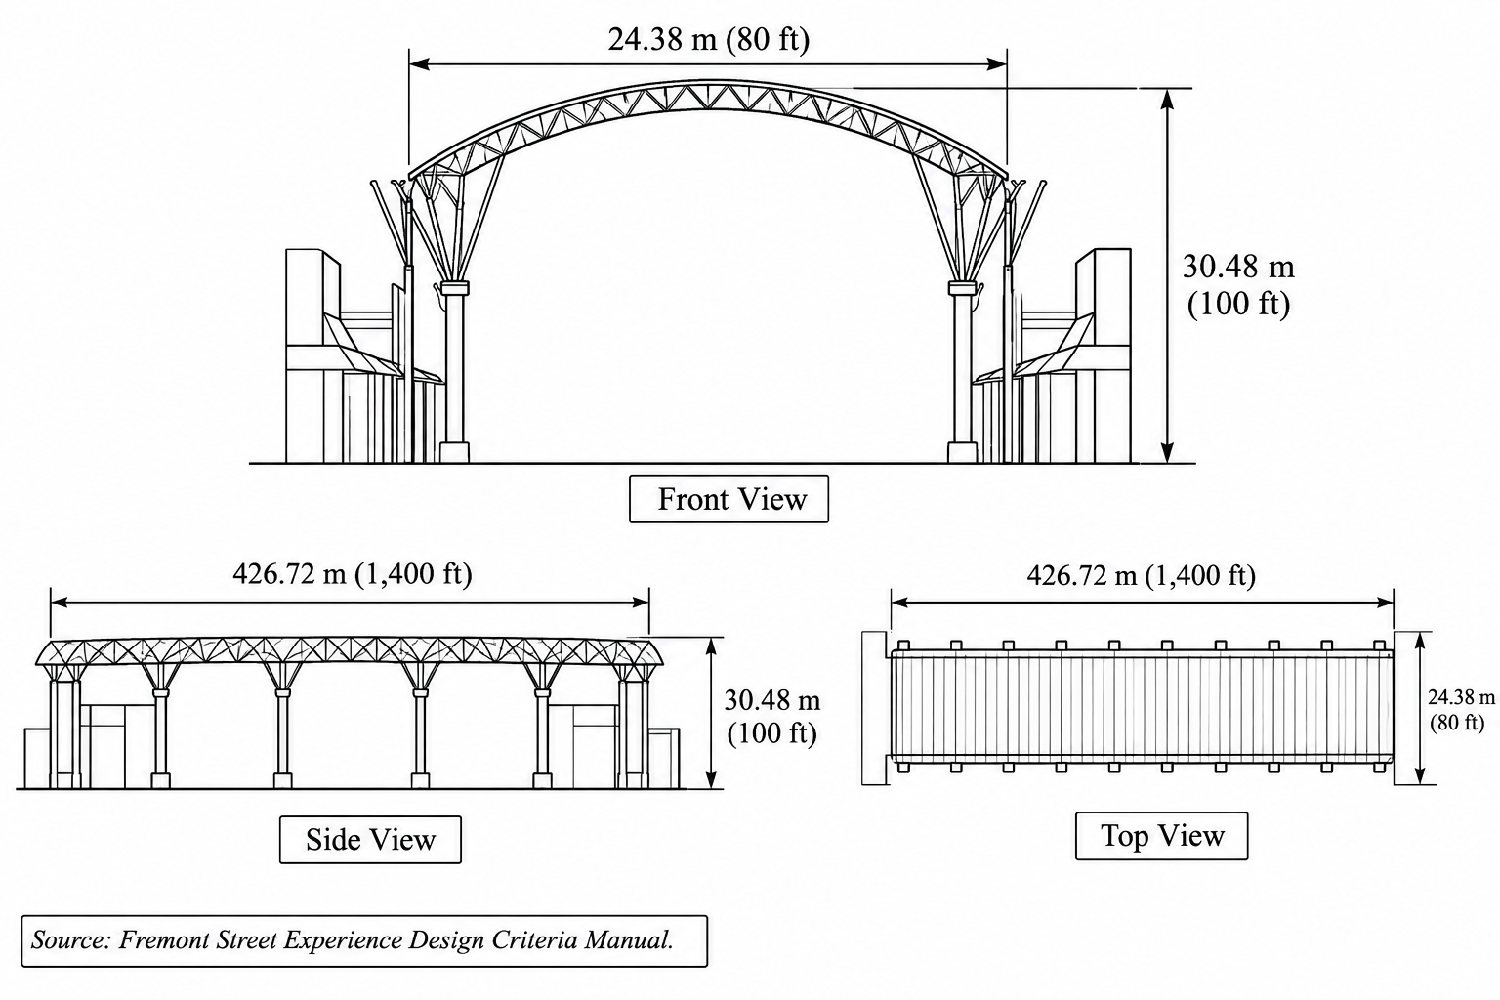
\includegraphics[width=\linewidth]{figures/32_fremont_context.pdf}\\[-1pt]
{\small\textbf{(a)} Fremont canopy context}
\end{minipage}\hfill
\begin{minipage}[t]{0.49\linewidth}
\centering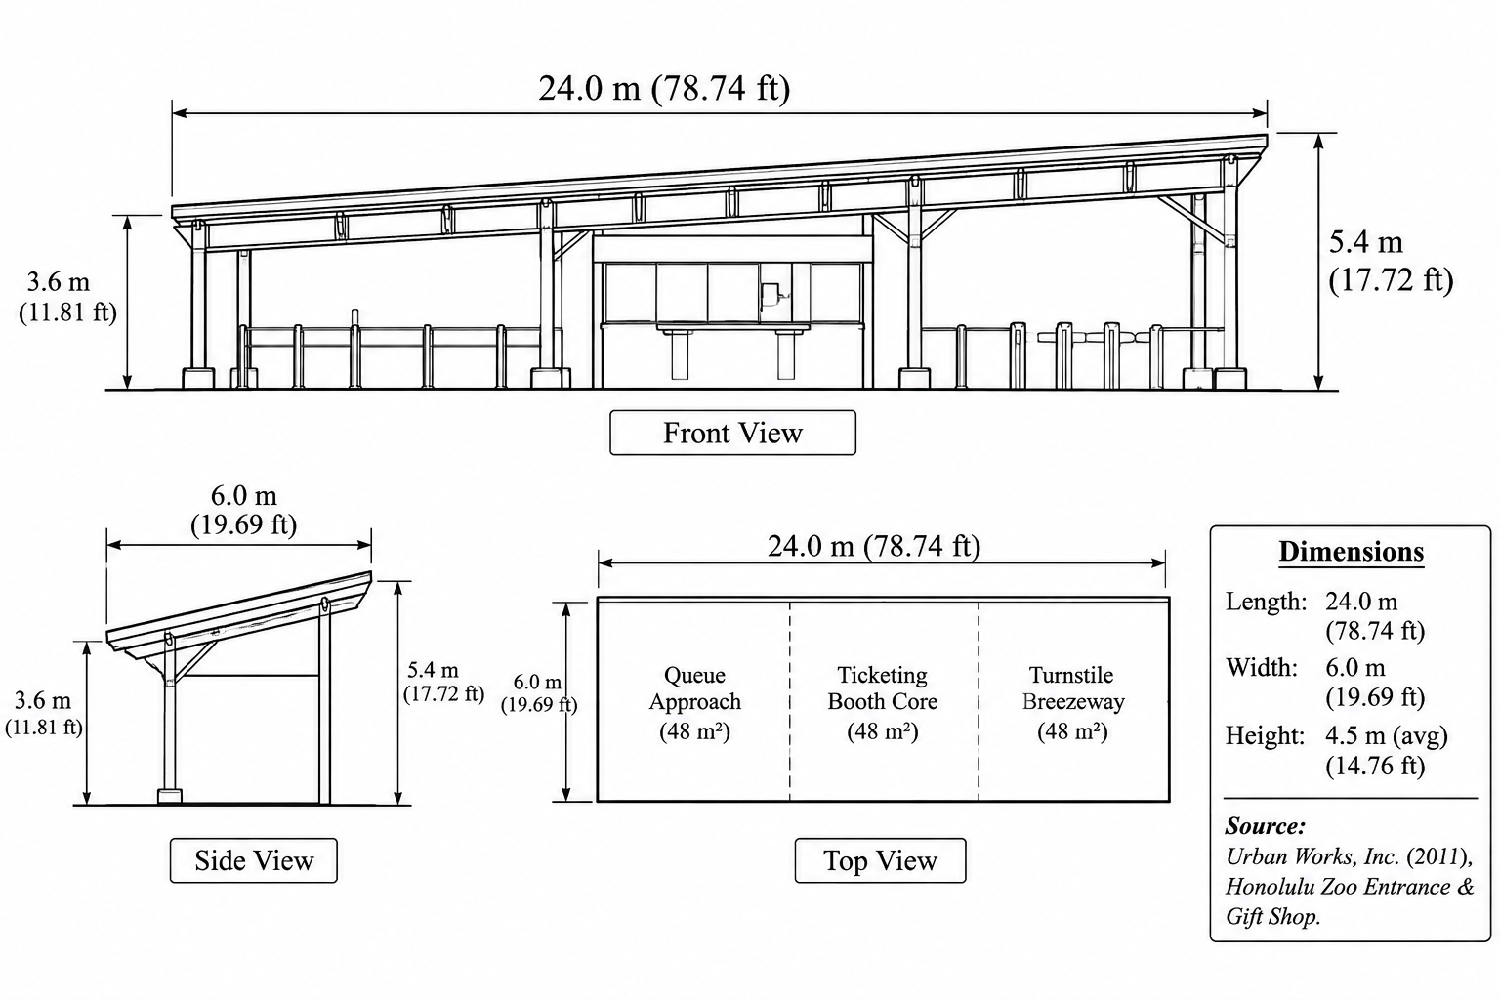
\includegraphics[width=\linewidth]{figures/33_honolulu_context.pdf}\\[-1pt]
{\small\textbf{(b)} Honolulu entrance context}
\end{minipage}
\caption{Supplied architectural schematics provide venue context. Their full-structure dimensions differ from the analytical service boundaries: Fremont uses the sourced $419.1$-m length and assumed $20$-m occupied width; Honolulu uses a $60$-m$^2$ public queue. Drawing dimensions are not substituted into the calculation.}
\label{fig:venue-context}
\end{figure}

\subsection{Transfer the physical kernel, then aggregate service}
We use the fixed-reservoir limit of the station model: outdoor $h,w,T_r$ are prescribed, while its integer allocation and coverage calculation are retained. Each unit uses the same wet-bulb-limited outlet, conservative local mixing and SET response as in Task 2. The three strip responses are averaged \emph{after} conversion to excess SET. Let $\delta_k=\frac13\sum_{j=1}^3[D_0-D(\Theta_{kj})]$ be the mean relief inside a complete footprint, and $\mathcal H_z=\int_0^H n_z(t)\,dt$ the zone's visitor-hours. Then
\begin{equation}
 u_{zk}=\mathcal H_z\frac{a_k}{A_z}\delta_k,\qquad
 U_s=\sum_{z,k}x_{zk}u_{zk},\qquad E_s=H\sum_{z,k}x_{zk}p_k.
\label{eq:venue-service}
\end{equation}
Time is measured in hours, giving $3210$ and $96$ visitor-hours in Fremont and Honolulu. Person-time coverage is $q_s=\sum_z\mathcal H_z\sum_k c_{zk}/\sum_z\mathcal H_z$. All installed units run throughout the four-hour period; water supply is counted once per unit. The disjoint-footprint condition in Eq.~\eqref{eq:coverage} prevents double-counting people.

This linear service structure also solves the efficiency-only allocation problem. For every positive-energy layout,
\begin{equation}
 \eta_s=\sum_{z,k}\frac{Hx_{zk}p_k}{E_s}\,
                  \frac{u_{zk}}{Hp_k}
 \ \le\ \max_{z,k}\frac{u_{zk}}{Hp_k}.
\label{eq:venue-bound}
\end{equation}
The bound is attained by one unit of the maximizing type in the maximizing zone whenever its footprint fits. It yields \textbf{$\FMaxEta$ in Fremont and $\HMaxEta$ in Honolulu} person$\cdot{}^\circ$C$\cdot$h/kWh, attained by A in Fremont's middle demand zone and A in the ticket queue. Their coverages are $0.33\%$ and $33.33\%$. Additional A units within the same zone tie while their footprints fit. This efficiency result uses the entire integer domain, without a service-coverage or cost threshold.

\subsection{Climate changes the relative value of the devices}
Table~\ref{tab:venue-results} compares the largest pure-type installations that fit each site. Honolulu admits three A units, two B units or one C unit: the last serves only two-thirds of the queue. Every unit's full power remains in the denominator.
\begin{table}[!ht]
\centering\small
\caption{Largest-fitting pure installations. Coverage $q$ is visitor-time weighted; $U$ has units person$\cdot{}^\circ$C$\cdot$h and $\eta=U/E$.}
\label{tab:venue-results}
\begin{tabular}{@{}llrrrr@{}}
\toprule
Venue & Plan & $q$ (\%) & $U$ & $E$ (kWh) & $\eta$\\
\midrule
Fremont & A419 & 99.99 & 4977.81 & 419.0 & 11.88\\
 & B279 & 99.91 & 6782.04 & 1339.2 & 5.06\\
 & C209 & 99.84 & 11951.71 & 2090.0 & 5.72\\
Honolulu & A3 & 100.00 & 143.12 & 3.0 & 47.71\\
 & B2 & 100.00 & 204.26 & 9.6 & 21.28\\
 & C1 & 66.67 & 206.30 & 10.0 & 20.63\\
\bottomrule
\end{tabular}
\end{table}


The wet-bulb temperatures are $\FTwb^\circ$C and $\HTwb^\circ$C. C's outlet drop reaches $\FCDrop^\circ$C in Fremont and $\HCDrop^\circ$C in Honolulu. At the dry site, C's larger temperature reduction and delivery profile outweigh its extra power relative to B; at the coastal site, B supplies more useful service per kWh than C. A retains the highest efficiency in both nominal cases. These rankings follow from local exposure and electricity together.



Honolulu's larger efficiency values also reflect its greater visitor density. To isolate the climate effect, we exchange $(T_a,\mathrm{RH},T_r,v_0)$ between sites while holding geometry, attendance and device counts fixed. The B--C order follows the weather tuple in both transfers. At Honolulu's density, A's efficiency changes from $\HMaxEta$ under its own weather to $\HWithFEta$ under Fremont's weather. Thus a high site-level $\eta$ cannot be attributed to favorable climate alone.

Natural wind also changes the marginal value of equipment: raising Fremont's background speed from $0.20$ to $0.80$ m/s changes the efficiency-maximizing type from A to C, with a new bound of $5.38$. The uncooled baseline SET falls from $33.77$ to $31.51^\circ$C. Extra fan speed brings less benefit when ambient air is already moving, whereas evaporative temperature reduction remains available.

\subsection{Controlled scaling and the finite-footprint limit}
For a fixed climate and unchanged local delivery, multiply each zone's area and visitor-hours by $\lambda$. With the original devices, each footprint contains the same number of people, so $U$ and $E$ remain constant while person-time coverage becomes $q/\lambda$. Replicating devices as well gives
\begin{equation}
 (A_z,\mathcal H_z,x_{zk})\mapsto
 (\lambda A_z,\lambda\mathcal H_z,\lambda x_{zk})
 \quad\Longrightarrow\quad
 (U,E,q,\eta)\mapsto(\lambda U,\lambda E,q,\eta).
\label{eq:venue-scale}
\end{equation}
Integer multipliers preserve feasible counts. For the Honolulu A3 reference, scaling from 60 to 480 m$^2$ with attendance at the same density leaves $\eta=\HMaxEta$. Three fixed fans reduce coverage from $100\%$ to $12.5\%$; 24 fans restore full coverage and raise four-hour electricity from 3 to 24 kWh. These are controlled similarity properties of the model, separating scale from climate.

\begin{figure}[!ht]
\centering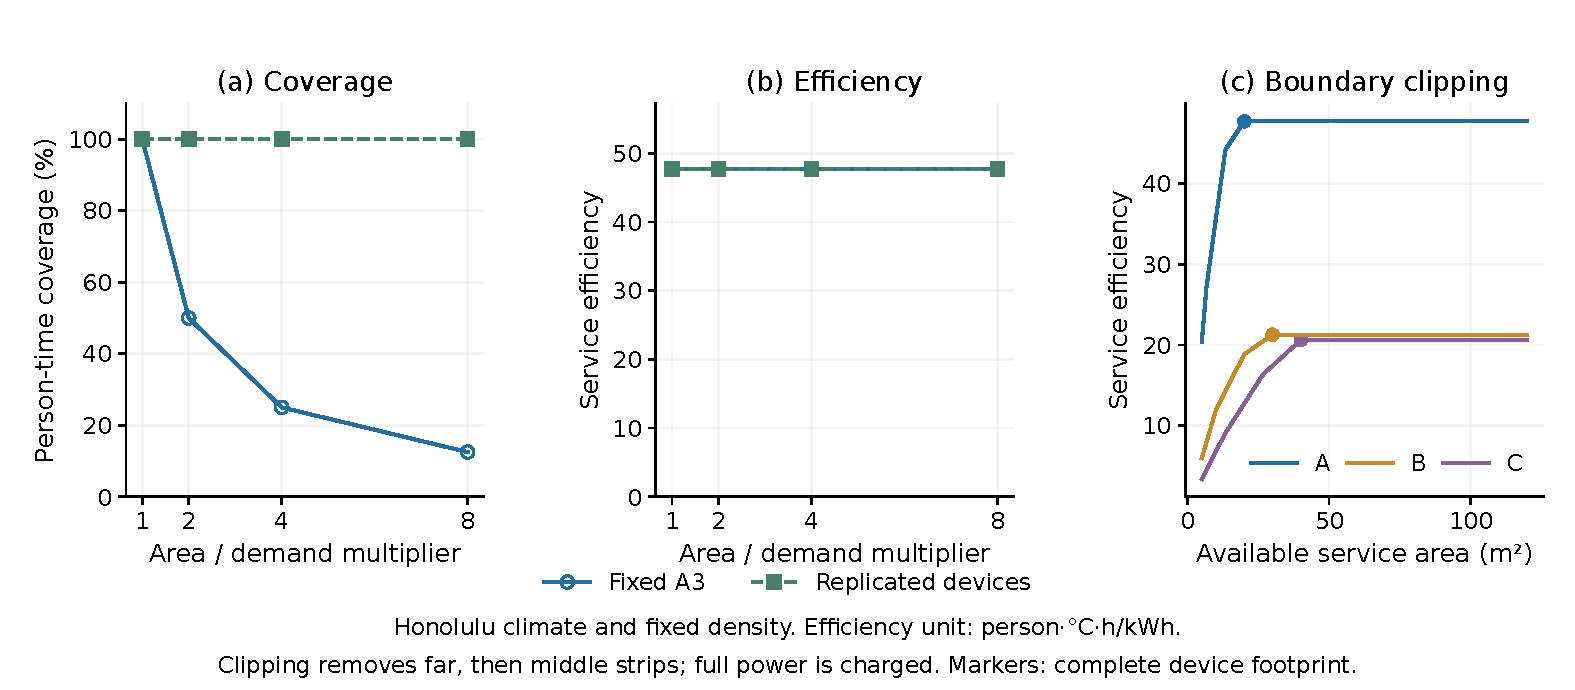
\includegraphics[width=0.96\linewidth]{figures/30_scale_transfer.pdf}
\caption{Controlled scale and boundary tests. Proportional deployment preserves efficiency and coverage; fixed equipment preserves efficiency but loses coverage. In the separate single-unit test, reducing available area clips the far delivery strip first, with the full unit power still charged.}
\label{fig:venue-scaling}
\end{figure}

Small spaces also expose a finite-footprint limit. We retain only the portions of the near, middle and far strips lying within the service boundary and recompute their area-weighted relief. The efficiency plateaus once a complete footprint fits; below that size, lost served area changes the result even at unchanged visitor density. Therefore the transferable characteristics are \textbf{occupied density, retained local delivery, wet-bulb depression and footprint fit}. Geometry sets who benefits; climate sets the benefit per exposed person. Matched-baseline identities, valid local air states and the scaling relations are checked against the exported calculations.
\FloatBarrier
